\documentclass{book}
\usepackage[spanish]{babel}
\usepackage[T1]{fontenc}
\usepackage[utf8]{inputenc}
\usepackage{amsmath, amssymb}
\usepackage{dsfont}
\usepackage{graphics}
\usepackage{cases}
\usepackage{graphicx}
\usepackage{pgf}
\usepackage{epsfig}
\usepackage{amssymb}
\usepackage{multirow}
\usepackage{amstext}
\usepackage[ruled,vlined,lined]{algorithm2e}
\usepackage{listings}
\usepackage{amsmath}
\usepackage{epic}
\usepackage{epsfig}
\usepackage{fontenc}
\usepackage{framed,color}
\usepackage{palatino, url, multicol}



\begin{document}

\chapter{Procesamiento del Lenguaje Natural}

El volumen de datos textuales digitalizados que se genera cada día es enorme (por ejemplo, la web, redes sociales, registros médicos, libros digitalizados). Por lo tanto, también crece la necesidad de traducir, analizar y gestionar esta avalancha de palabras y texto.

El procesamiento del lenguaje natural (PLN) es el campo que se encarga de diseñar métodos y algoritmos que toman como entrada o producen como salida datos de \textbf{lenguaje natural} no estructurado \cite{goldberg2017neural}. El PLN se centra en el diseño y análisis de algoritmos computacionales y representaciones para procesar el lenguaje humano \cite{jacobbook}.





Una tarea común de PLN es el Reconocimiento de Entidades Nombradas (NER, por sus siglas en inglés). Por ejemplo:

\begin{figure}[h]
	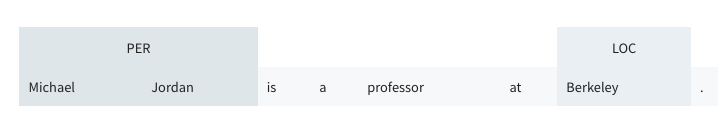
\includegraphics[scale=0.4]{pics/NER.png}
	\caption{Reconocimiento de Entidades Nombradas}
\end{figure}

El lenguaje humano es altamente ambiguo, como en las frases: "Comí pizza con amigos", "Comí pizza con aceitunas" o "Comí pizza con un tenedor". Además, el lenguaje está en constante cambio y evolución, como ocurre con los hashtags en Twitter.

\section{PLN y Lingüística Computacional}
PLN suele confundirse con otra disciplina hermana llamada Lingüística Computacional (LC). Si bien ambas están estrechamente relacionadas, tienen un foco distinto. La LC busca responder preguntas fundamentales sobre el lenguaje mediante el uso de la computación, es decir, cómo entendemos el lenguaje, cómo producimos lenguaje o cómo aprendemos lenguaje. Mientras que en PLN el foco está en resolver problemas específicos, tales como las transcripción automática del habla, la traducción automática, la extracción de información de documentos y el análisis de opiniones en redes sociales. Es importante señalar que en PLN, el éxito de una solución se mide en base métricas concretas (Ej: qué tan similar es la traducción automática a una hecha por un humano) independientemente si el modelo hace uso de alguna teoría lingüística.



El procesamiento del lenguaje natural (PLN) desarrolla métodos para resolver problemas prácticos relacionados con el lenguaje \cite{JohnsonMLSS}.

Algunos ejemplos son:

\begin{itemize}
  \item Reconocimiento automático del habla.
  \item Traducción automática.
  \item Extracción de información de documentos.
\end{itemize}

La lingüística computacional (LC) estudia los procesos computacionales subyacentes al lenguaje (humano).

\begin{itemize}
  \item ¿Cómo comprendemos el lenguaje?
  \item ¿Cómo producimos el lenguaje?
  \item ¿Cómo aprendemos el lenguaje?
\end{itemize}

El PLN y la LC utilizan métodos y modelos similares.


Aunque existe una superposición sustancial, hay una diferencia importante en el enfoque. La LC se centra en la lingüística respaldada por métodos computacionales (similar a la biología computacional o la astronomía computacional). En lingüística, el lenguaje es el objeto de estudio. El PLN se centra en resolver tareas bien definidas relacionadas con el lenguaje humano (como la traducción, la respuesta a consultas, las conversaciones). Si bien los conocimientos lingüísticos fundamentales pueden ser cruciales para realizar estas tareas, el éxito se mide en función de si y cómo se logra el objetivo (según una métrica de evaluación) \cite{jacobbook}.



El procesamiento del lenguaje natural y la lingüística computacional están estrechamente relacionados y se superponen en muchos aspectos. Ambos campos utilizan métodos y modelos similares para abordar problemas relacionados con el lenguaje humano. Sin embargo, la diferencia principal radica en el enfoque: la lingüística computacional se centra en la lingüística respaldada por métodos computacionales, mientras que el procesamiento del lenguaje natural se centra en resolver tareas prácticas relacionadas con el lenguaje. Ambos campos son fundamentales para comprender y aprovechar el poder del lenguaje humano en la era digital.


\section{Niveles de descripción lingüística}

El campo de la \textbf{descripción lingüística} abarca diferentes niveles:

\begin{itemize}
  \item \textbf{Fonética y fonología:} estudio de los sonidos del habla.
  \item \textbf{Morfología:} estudio de la estructura de las palabras.
  \item \textbf{Sintaxis:} estudio de la estructura de las oraciones.
  \item \textbf{Semántica:} estudio del significado de las palabras y oraciones.
  \item \textbf{Pragmática:} estudio del uso del lenguaje en el contexto.
\end{itemize}

El PLN puede abordar tareas en cada uno de estos niveles, pero a menudo se enfoca en niveles más altos de representación y comprensión.




\subsection{Fonética}

La fonética es la rama de la lingüística que se ocupa del estudio de los sonidos del lenguaje. Examina los órganos utilizados en la producción de sonidos, como la boca, la lengua, la garganta, la nariz, los labios y el paladar. Los sonidos del lenguaje se dividen en vocales y consonantes. Las vocales se producen con poca restricción del flujo de aire desde los pulmones, mientras que las consonantes implican alguna restricción o cierre en el tracto vocal \cite{JohnsonMLSS, fromkin2018introduction}. Además, el Alfabeto Fonético Internacional (AFI) proporciona una notación alfabética para representar los sonidos fonéticos.

\subsection{Fonología}

La fonología se centra en el estudio de cómo los sonidos del habla forman patrones y construyen significado. Los fonemas son las unidades básicas de sonido que diferencian el significado de las palabras. Por ejemplo, en inglés, la "p" y la "b" son fonemas distintos porque cambian el significado de las palabras en las que se encuentran. La fonología también examina las variaciones en la pronunciación de los sonidos en diferentes contextos y dialectos \cite{fromkin2018introduction}.

\subsection{Morfología}

La morfología se ocupa del estudio de la estructura interna de las palabras. Los morfemas son las unidades mínimas de significado que componen las palabras. Por ejemplo, en la palabra "deshacer", los morfemas son "des-", "hacer" y "-er". La morfología también se interesa por los procesos de formación de palabras, como la derivación, donde se agregan prefijos o sufijos a una palabra existente para formar una nueva palabra con un significado diferente \cite{JohnsonMLSS}.

\begin{itemize}
\item La morfología estudia la estructura de las palabras (por ejemplo, re+estructur+ando, in+olvid+able) \cite{JohnsonMLSS}
\item Morfema: el término lingüístico para la unidad más elemental de forma gramatical \cite{fromkin2018introduction}. Por ejemplo, morfología = morf + ología (la ciencia de).
\item Morfología derivativa: proceso de formar una nueva palabra a partir de una palabra existente, a menudo mediante la adición de un prefijo o sufijo.
\item La morfología derivativa exhibe una estructura jerárquica. Ejemplo: re+vital+iz+ación
\begin{figure}[h]
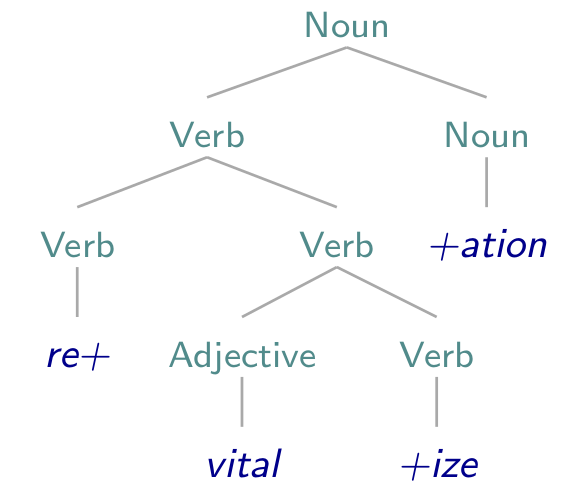
\includegraphics[scale = 0.2]{pics/morphology.png}
\end{figure}
\item El sufijo generalmente determina la categoría sintáctica (part-of-speech) de la palabra derivada.
\end{itemize}

\subsection{Sintaxis}

La sintaxis es el estudio de cómo las palabras se combinan para formar frases y oraciones gramaticales. Examina las reglas y estructuras que determinan la organización de las palabras en una oración y cómo influyen en el significado. La sintaxis también se ocupa de la relación entre las palabras y las funciones que desempeñan dentro de una oración. Por ejemplo, en la oración "El perro persigue al gato", "el perro" es el sujeto, "persigue" es el verbo y "al gato" es el complemento directo \cite{JohnsonMLSS}.

\begin{itemize}
\item La sintaxis estudia las formas en que las palabras se combinan para formar frases y oraciones \cite{JohnsonMLSS}
\begin{figure}[h]
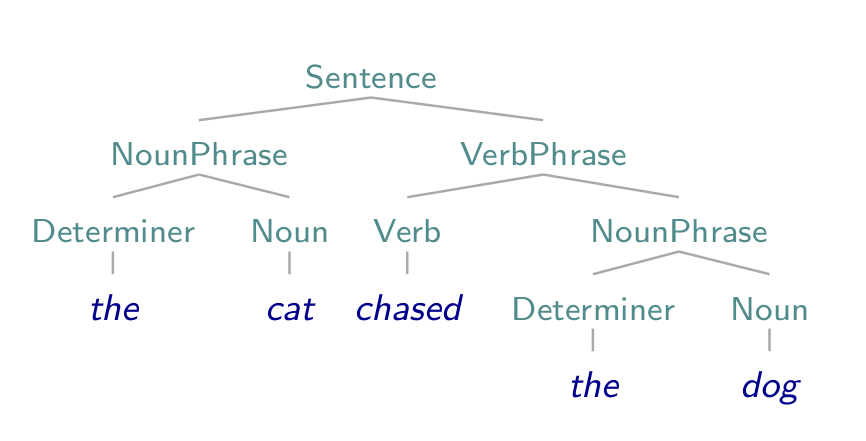
\includegraphics[scale = 0.3]{pics/parseTree1.png}
\end{figure}
\item El análisis sintáctico ayuda a identificar \textbf{quién hizo qué a quién}, un paso clave para comprender una oración.
\end{itemize}


\subsection{Semántica}

La semántica es el estudio del significado de las palabras, frases y oraciones, examinando cómo se construye e interpreta este significado en el contexto del lenguaje. Además, la semántica se interesa por los roles semánticos, que indican la función de cada entidad en una oración. Por ejemplo, en la oración "El niño cortó la cuerda con una navaja", "el niño" es el agente, "la cuerda" es el tema y "una navaja" es el instrumento \cite{JohnsonMLSS}.

La semántica se enfoca en el significado de las palabras, frases y oraciones. Estudia cómo se construye e interpreta este significado en el contexto del lenguaje. Además, dentro de la semántica, se analizan los roles semánticos, los cuales indican la función que desempeña cada entidad en una oración. Por ejemplo, en la oración "El niño cortó la cuerda con una navaja", se identifican distintos roles semánticos: "el niño" como el agente, "la cuerda" como el tema y "una navaja" como el instrumento utilizado \cite{JohnsonMLSS}.


En resumen:
\begin{itemize}
\item La semántica estudia el significado de las palabras, frases y oraciones \cite{JohnsonMLSS}.
\item Dentro de la semántica, se analizan los roles semánticos, que indican el papel desempeñado por cada entidad en una oración.
\item Algunos ejemplos de roles semánticos son: \textcolor[rgb]{0.00,0.00,1.00}{\textbf{agente}} (la entidad que realiza la acción), \textcolor[rgb]{1.00,0.00,0.00}{\textbf{tema}} (la entidad involucrada en la acción) y \textcolor[rgb]{0.00,1.00,0.00}{\textbf{instrumento}} (otra entidad utilizada por el agente para llevar a cabo la acción).
\item En la oración "El niño cortó la cuerda con una navaja", se puede identificar el agente como \textcolor[rgb]{0.00,0.00,1.00}{\textbf{el niño}}, el tema como \textcolor[rgb]{1.00,0.00,0.00}{\textbf{la cuerda}} y el instrumento como \textcolor[rgb]{0.00,1.00,0.00}{\textbf{una navaja}}.
\item Además de los roles semánticos, la semántica también abarca las relaciones léxicas, que son las relaciones entre diferentes palabras \cite{yule2016study}.
\item Algunos ejemplos de relaciones léxicas incluyen la sinonimia (conceal/hide), la antonimia (shallow/deep) y la hiponimia (perro/animal).
\end{itemize}


\subsection{Pragmática}

La pragmática se centra en cómo el contexto influye en la interpretación y el significado de las expresiones lingüísticas. Examina cómo se utilizan las expresiones lingüísticas en situaciones reales y cómo los hablantes interpretan el significado implícito. Por ejemplo, la oración "Hace frío aquí" puede interpretarse como una sugerencia implícita de cerrar las ventanas \cite{fromkin2018introduction}.


\section{Procesamiento del Lenguaje Natural y Aprendizaje Automático}

Comprender y producir el lenguaje computacionalmente es extremadamente complejo.  La tecnología más exitosa actualmente para abordar PLN es el aprendizaje automático supervisado que consiste en una familia de algoritmos que “aprenden” a construir la respuesta del problema en cuestión en base a encontrar patrones en datos de entrenamiento etiquetados. Por ejemplo, si queremos tener un modelo que nos diga si un tweet tiene un sentimiento positivo o negativo respecto a un producto, primero necesito  etiquetar manualmente un conjunto de tweets con su sentimiento asociado. Luego debo entrenar un algoritmo de aprendizaje sobre estos datos para poder predecir de manera automática el sentimiento asociado a tweets desconocidos. Como se podrán imaginar, el etiquetado de datos es una parte fundamental de la solución y puede ser un proceso muy costoso, especialmente cuando se requiere conocimiento especializado para definir la etiqueta.

Aunque los seres humanos somos grandes usuarios del lenguaje, también somos muy malos para comprender y describir formalmente las reglas que rigen el lenguaje.

Entender y producir lenguaje utilizando computadoras es altamente desafiante. Los métodos más conocidos para lidiar con datos de lenguaje se basan en el aprendizaje automático supervisado.

El aprendizaje automático supervisado consiste en intentar inferir patrones y regularidades a partir de un conjunto de pares de entrada y salida preanotados (también conocido como conjunto de datos de entrenamiento).

\paragraph{Conjunto de Datos de Entrenamiento: Datos de NER CoNLL-2003}

Cada línea contiene un token, una etiqueta de parte de la oración, una etiqueta de sintagma y una etiqueta de entidad nombrada.
\begin{center}
\begin{verbatim}
U.N.         NNP  I-NP  I-ORG
official     NN   I-NP  O
Ekeus        NNP  I-NP  I-PER
heads        VBZ  I-VP  O
for          IN   I-PP  O
Baghdad      NNP  I-NP  I-LOC
.            .    O     O
\end{verbatim}
\end{center}

\footnotemark{Fuente: \url{https://www.clips.uantwerpen.be/conll2003/ner/}}

\section{Desafíos del Lenguaje}

Existen tres propiedades desafiantes del lenguaje: la discreción, la composicionalidad y la dispersión.

\textbf{Discreción}: no podemos inferir la relación entre dos palabras a partir de las letras que las componen (por ejemplo, hamburguesa y pizza).

\textbf{Composicionalidad}: el significado de una oración va más allá del significado individual de sus palabras.

\textbf{Dispersión}: la forma en que las palabras (símbolos discretos) pueden combinarse para formar significados es prácticamente infinita.



\section{Ejemplo de tareas NLP}


\paragraph{Clasificación de temas}

La clasificación de temas es una tarea de Procesamiento del Lenguaje Natural (PLN) en la cual se asigna a un documento una de varias categorías, como deportes, política, cotilleos o economía. Las palabras presentes en los documentos brindan pistas importantes sobre su tema. Sin embargo, redactar reglas para esta tarea es un desafío debido a la complejidad del lenguaje. La anotación de datos, en la cual los lectores clasifican los documentos por temas, puede ayudar a generar conjuntos de datos de entrenamiento para algoritmos de aprendizaje automático supervisado. Estos algoritmos aprenden patrones de uso de palabras que facilitan la categorización de los documentos.

\begin{itemize}
\item Clasificar un documento en una de las cuatro categorías: Deportes, Política, Cotilleos y Economía.
\item Las palabras en los documentos proporcionan indicios muy sólidos.
\item ¿Qué palabras brindan qué indicios?
\item Elaborar reglas para esta tarea resulta bastante desafiante.
\item No obstante, los lectores pueden categorizar fácilmente varios documentos según su tema (anotación de datos).
\item Un algoritmo de aprendizaje automático supervisado puede identificar los patrones de uso de palabras que ayudan a categorizar los documentos.
\end{itemize}
\paragraph{Análisis de Sentimiento}

El análisis de sentimientos se refiere a la aplicación de técnicas de Procesamiento del Lenguaje Natural (PLN) para identificar y extraer información subjetiva de conjuntos de datos textuales. Un desafío común en el análisis de sentimientos es la clasificación de la polaridad a nivel de mensaje (MPC), donde las frases se clasifican automáticamente en categorías positivas, negativas o neutrales. Las soluciones más avanzadas utilizan modelos de aprendizaje automático supervisado entrenados con ejemplos anotados manualmente.

En este tipo de clasificación, es habitual emplear el aprendizaje supervisado, siendo las Máquinas de Vectores de Soporte (SVM) una opción popular. El objetivo de las SVM es encontrar un hiperplano que separe las clases con el margen máximo, logrando la mejor separación entre las clases positivas, negativas y neutrales \cite{jacobbook}.

\begin{itemize}
  \item Aplicación de técnicas de \textbf{PLN} para identificar y extraer información subjetiva de conjuntos de datos textuales.
  \item Clasificación automática de frases en las categorías \textcolor[rgb]{0.00,0.00,1.00}{\textbf{positiva}}, \textcolor[rgb]{1.00,0.00,0.00}{\textbf{negativa}} o \textcolor[rgb]{0.00,1.00,0.00}{\textbf{neutral}}.

     \begin{figure}[h]
        	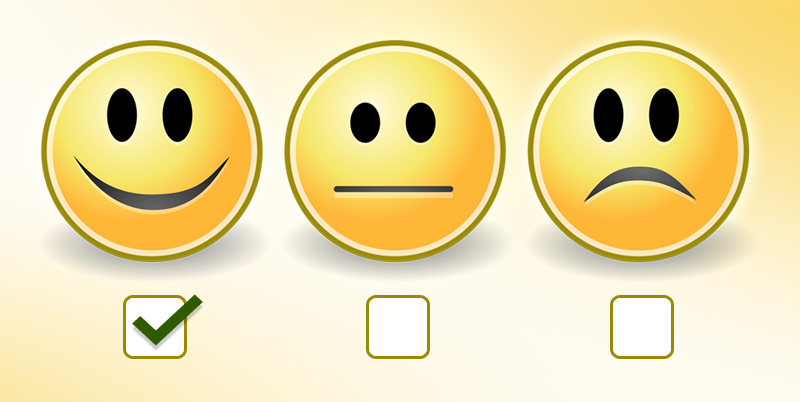
\includegraphics[scale = 0.15]{pics/sent.png}
        \end{figure}

  \item Las soluciones más avanzadas emplean modelos de aprendizaje automático \textbf{supervisado}, entrenados con ejemplos \textbf{anotados manualmente} \cite{Mohammad2013}.
\end{itemize}


\begin{figure}[h]
        	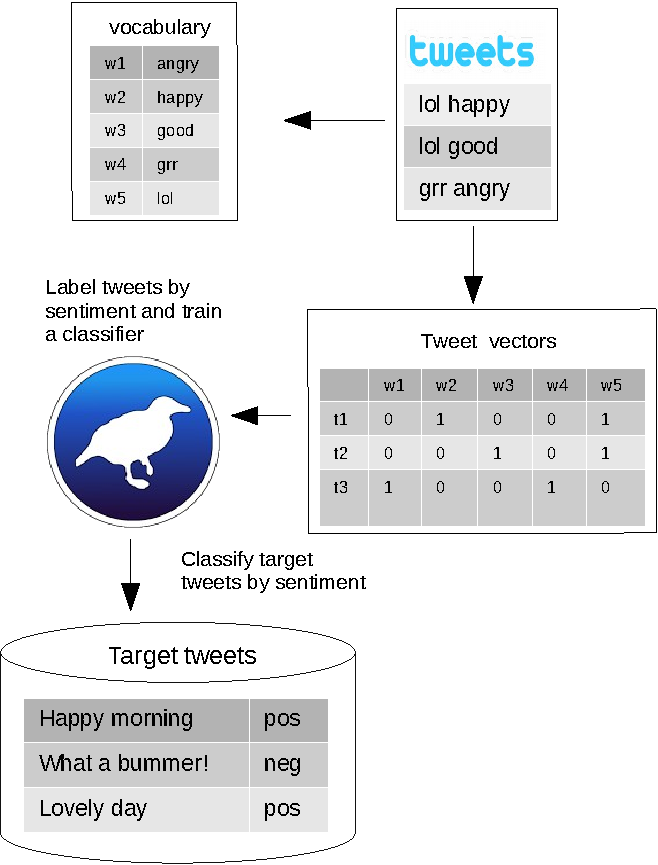
\includegraphics[scale = 0.5]{pics/bagOfwordsClassification.pdf}
        \end{figure}


\begin{itemize}


\item Idea: Encontrar un hiperplano que separe las clases con el margen máximo (mayor separación).

     \begin{figure}[h]
        	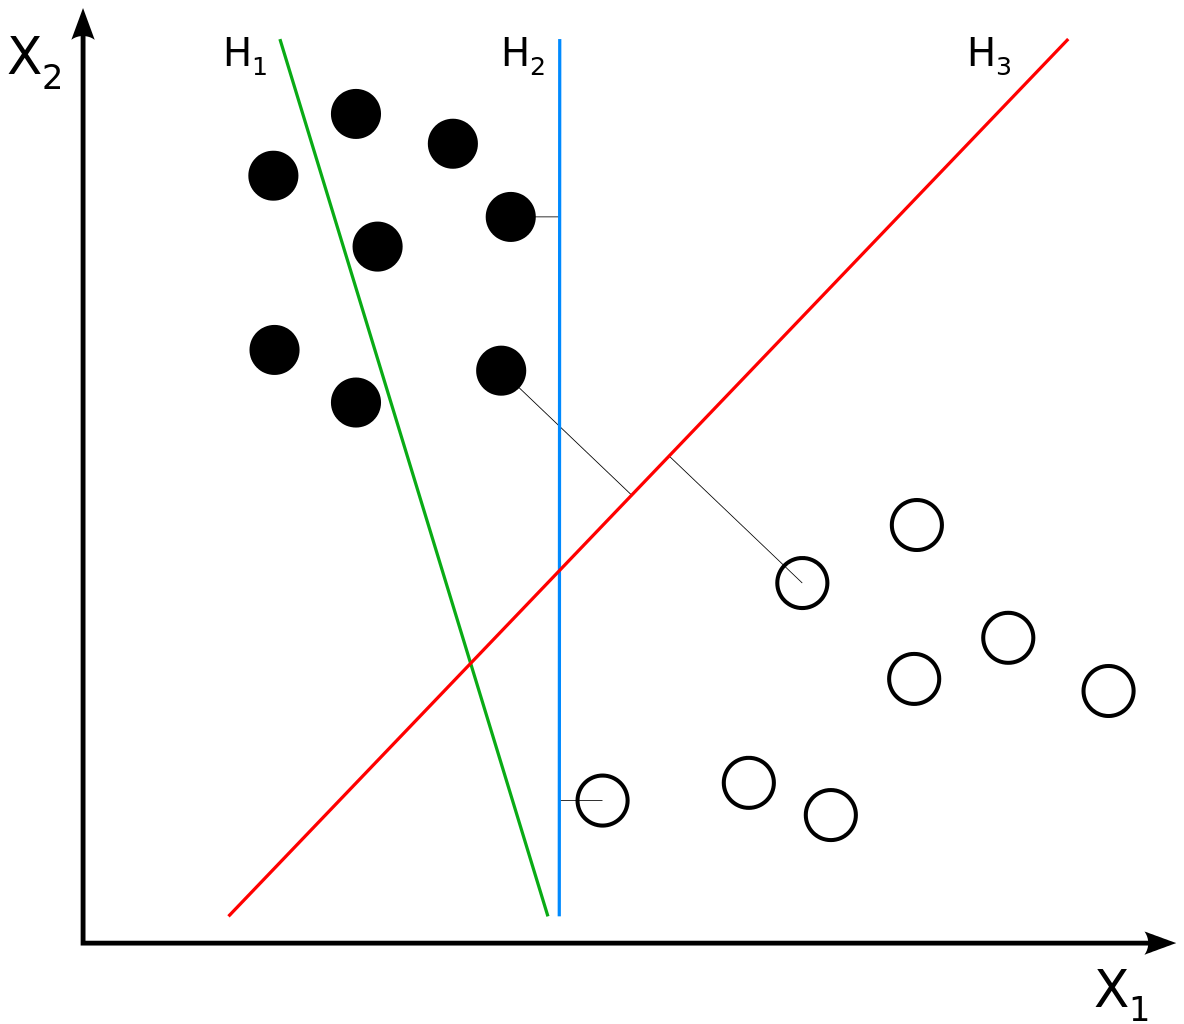
\includegraphics[scale = 0.15]{pics/SVM.png}
        \end{figure}

\item $H_3$ separa las clases con el margen máximo.

\end{itemize}


\subsection{Lingüística y Procesamiento del Lenguaje Natural (PNL)}

El conocimiento de las estructuras lingüísticas es fundamental para el diseño de características y el análisis de errores en el Procesamiento del Lenguaje Natural (PNL). Los enfoques de aprendizaje automático en PNL se basan en características que describen y generalizan las instancias de uso del lenguaje. El conocimiento lingüístico orienta la selección y el diseño de estas características, ayudando al algoritmo de aprendizaje automático a encontrar correlaciones entre el uso del lenguaje y las etiquetas objetivo \cite{bender2013linguistic}.

\begin{itemize}
  \item El conocimiento de las estructuras lingüísticas es importante para el diseño de características y el análisis de errores en PNL \cite{bender2013linguistic}.
  \item Los enfoques de aprendizaje automático en PNL requieren características que puedan describir y generalizar el uso del lenguaje.
  \item El objetivo es guiar al algoritmo de aprendizaje automático para encontrar correlaciones entre el uso del lenguaje y el conjunto de etiquetas objetivo.
  \item El conocimiento sobre las estructuras lingüísticas puede influir en el diseño de características para los enfoques de aprendizaje automático en PNL.
\end{itemize}

El PNL plantea diversos desafíos, como los costos de anotación, las variaciones de dominio y la necesidad de actualizaciones continuas. La anotación manual requiere mucho trabajo y tiempo. Las variaciones de dominio implican aprender patrones diferentes para diferentes corpus de texto. Los modelos entrenados en un dominio pueden no funcionar bien en otro. Además, los modelos de PNL pueden volverse obsoletos a medida que el uso del lenguaje evoluciona con el tiempo.




\section{Desafíos en el Procesamiento del Lenguaje Natural (PNL)}

\begin{itemize}
   \item \textbf{Costos de Anotación}: la anotación manual es \textbf{laboriosa} y \textbf{consume mucho tiempo}.
   \item \textbf{Variaciones de Dominio}: el patrón que queremos aprender puede variar de un corpus a otro (por ejemplo, deportes, política).

   \item ¡Un modelo entrenado con datos anotados de un dominio no necesariamente funcionará en otro!
   \item Los modelos entrenados pueden quedar desactualizados con el tiempo (por ejemplo, nuevos hashtags).
\end{itemize}

\paragraph{Variación de Dominio en el Análisis de Sentimiento}
\begin{enumerate}
   \item Para mí, la cola era bastante \textcolor[rgb]{0.00,0.00,1.00}{\textbf{pequeña}} y solo tuve que esperar unos 20 minutos, ¡pero valió la pena! :D @raynwise
   \item Extraña espacialidad en Stuttgart. La habitación del hotel es tan \textcolor[rgb]{1.00,0.00,0.00}{\textbf{pequeña}} que apenas puedo moverme, pero los alrededores son inhumanamente vastos y largos bajo construcción.
\end{enumerate}

\paragraph{Superando los costos de anotación de datos}
Supervisión Distant:
\begin{itemize}
   \item Etiquetar automáticamente datos no etiquetados (\textbf{API de Twitter}) utilizando un método heurístico.
   \item \textbf{Enfoque de Anotación de Emoticonos (EAA)}: los tweets con emoticonos positivos \textcolor[rgb]{0.00,0.00,1.00}{\textbf{:)}} o negativos \textcolor[rgb]{1.00,0.00,0.00}{\textbf{:(}} se etiquetan según la polaridad indicada por el emoticono~\cite{Read2005}.
   \item El emoticono se \textbf{elimina} del contenido.
   \item Este enfoque también se ha ampliado utilizando hashtags como \#anger y emojis.
   \item No es trivial encontrar técnicas de supervisión distante para todo tipo de problemas de PNL.
\end{itemize}

\paragraph{Crowdsourcing}
\begin{itemize}
   \item Confiar en servicios como \textbf{Amazon Mechanical Turk} o \textbf{Crowdflower} para solicitar a la \textbf{multitud} que anote datos.
   \item Esto puede resultar costoso.
   \item Es difícil garantizar la calidad de las anotaciones.
\end{itemize}

\section{Estudio de caso: Clasificación de sentimientos en tweets}

\begin{itemize}
   \item En 2013, el taller de Evaluación Semántica (SemEval) organizó la tarea de "Análisis de sentimientos en Twitter" \cite{Semeval2013}.
   \item La tarea se dividió en dos sub-tareas: el nivel de expresión y el nivel del mensaje.
   \item Nivel de expresión: se centró en determinar la polaridad del sentimiento de un mensaje según una entidad marcada dentro de su contenido.
   \item Nivel del mensaje: se debía determinar la polaridad según el mensaje en general.
   \item Los organizadores lanzaron conjuntos de datos de entrenamiento y prueba para ambas tareas \cite{Semeval2013}.
\end{itemize}

\paragraph{El sistema NRC}
\begin{itemize}
   \item El equipo que logró el mejor rendimiento en ambas tareas, entre 44 equipos, fue el equipo \emph{NRC-Canada} \cite{Mohammad2013}.
   \item El equipo propuso un enfoque supervisado utilizando un clasificador SVM lineal con las siguientes características hechas a mano para representar los tweets:
   \begin{enumerate}
      \item N-gramas de palabras.
      \item N-gramas de caracteres.
      \item Etiquetas de partes del discurso.
      \item Agrupaciones de palabras entrenadas con el método de agrupamiento de Brown \cite{brown1992class}.
      \item El número de palabras alargadas (palabras con un carácter repetido más de dos veces).
      \item El número de palabras con todas las letras en mayúscula.
      \item La presencia de emoticonos positivos o negativos.
      \item El número de negaciones individuales.
      \item El número de secuencias contiguas de puntos, signos de interrogación y signos de exclamación.
      \item Características derivadas de lexicones de polaridad \cite{Mohammad2013}. Dos de estos lexicones se generaron utilizando el método PMI a partir de tweets anotados con hashtags y emoticonos.
   \end{enumerate}
\end{itemize}

\section{Ingeniería de características y Aprendizaje Profundo}

\begin{itemize}
   \item Hasta 2014, la mayoría de los sistemas de PNL de última generación se basaban en ingeniería de características + modelos de aprendizaje automático superficiales (por ejemplo, SVM, HMM).
   \item Diseñar las características de un sistema de PNL ganador requiere mucho conocimiento específico del dominio.
   \item El sistema NRC se construyó antes de que el aprendizaje profundo se hiciera popular en PNL.
   \item Por otro lado, los sistemas de Aprendizaje Profundo se basan en redes neuronales para aprender automáticamente buenas representaciones.
\end{itemize}

\paragraph{Ingeniería de características y Aprendizaje Profundo}

\begin{figure}[h]
   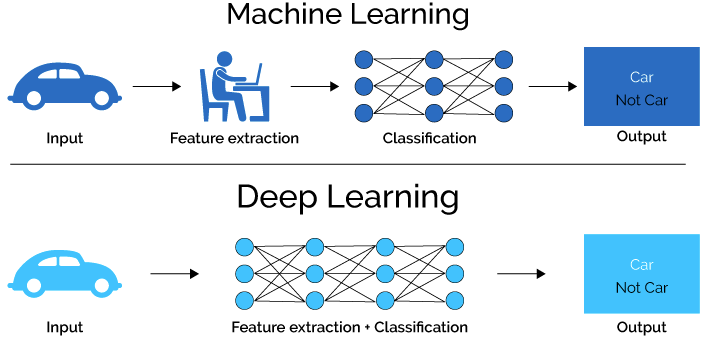
\includegraphics[scale = 0.25]{pics/MLvsDL.png}
\end{figure}

\begin{itemize}
   \item El Aprendizaje Profundo proporciona resultados de última generación en la mayoría de las tareas de PNL.
   \item Grandes cantidades de datos de entrenamiento y máquinas GPU

 multicore más rápidas son clave en el éxito del aprendizaje profundo.
   \item Las \textbf{redes neuronales} y las \textbf{incrustaciones de palabras} desempeñan un papel fundamental en los modelos modernos de PNL.

\end{itemize}

\paragraph{Aprendizaje Profundo y Conceptos Lingüísticos}
\begin{itemize}
   \item Si los modelos de aprendizaje profundo pueden aprender representaciones automáticamente, ¿siguen siendo útiles los conceptos lingüísticos (por ejemplo, sintaxis, morfología)?
   \item Algunos defensores del aprendizaje profundo argumentan que estas propiedades lingüísticas inferidas y diseñadas manualmente no son necesarias, y que la red neuronal aprenderá estas representaciones intermedias (o equivalentes o mejores) por sí misma \cite{goldberg2016primer}.
   \item Aún no hay un consenso definitivo al respecto.
   \item Goldberg cree que muchos de estos conceptos lingüísticos pueden ser inferidos por la red por sí misma si se le proporciona suficiente cantidad de datos.
   \item Sin embargo, en muchos otros casos no disponemos de suficientes datos de entrenamiento para la tarea que nos interesa, y en estos casos proporcionar a la red los conceptos generales más explícitos puede ser muy valioso.
\end{itemize}

\section{Historia}

Los orígenes de PLN se remontan a los años 50 con el famoso test de Alan Turing: una máquina será considerada inteligente cuando sea capaz de conversar con una persona sin que esta pueda determinar si está hablando con una máquina o un ser humano. A lo largo de su historia la disciplina ha tenido tres grandes períodos: 1) el racionalismo, 2) el empirismo, y 3) el aprendizaje profundo [Deng y Liu, 2018] que describimos a continuación.

El racionalismo abarca desde 1950 a 1990, donde las soluciones consistían en diseñar reglas manuales para incorporar mecanismos de conocimiento y razonamiento. Un ejemplo emblemático es el agente de conversación (o chatbot) ELIZA desarrollado por Joseph Weizenbaum que simulaba  un psicoterapeuta rogeriano. Luego, a partir de la década de los 90s, el diseño de métodos estadísticos y de aprendizaje automático construidos sobre corpus llevan a PLN hacia un enfoque empirista. Las reglas ya no se construyen sino que se “aprenden” a partir de datos etiquetados.  Algunos modelos representativos de esta época son los filtros de spam basados en modelos lineales, las cadenas de Markov ocultas para la extracción de categorías sintácticas y los modelos probabilísticos de IBM para la traducción automática. Estos modelos se caracterizaban por ser poco profundos en su estructura de parámetros y por depender de características manualmente diseñadas para representar la entrada.

A partir del año 2010, las redes neuronales artificiales, que son una familia de modelos de aprendizaje automático, comienzan a mostrar resultados muy superiores en varias tareas emblemáticas de PLN [Collobert et al., 2011]. La idea de estos modelos es representar la entrada (el texto) con una jerarquía de parámetros (o capas) que permiten encontrar representaciones idóneas para la tarea en cuestión, proceso al cual se refiere como “aprendizaje profundo”. Estos modelos se caracterizan por tener muchos más parámetros que los modelos anteriores (superando la barrera del millón en algunos casos) y requerir grandes volúmenes de datos para su entrenamiento. Una gracia de estos modelos es que pueden ser pre-entrenados con texto no etiquetado como libros, Wikipedia, texto de redes sociales y de la Web para encontrar representaciones iniciales de palabras y oraciones (a lo que conocemos como word embeddings),  las cuales pueden ser posteriormente adaptadas para la tarea objetivo donde sí se tienen datos etiquetados (Proceso conocido como transfer learning). Aquí destacamos modelos como Word2Vec [Mikolov 2013], BERT  [Devlin 2018] y GPT-3  [Brown 2020].

Este tipo de modelos ha ido perfeccionándose en los últimos años, llegando a obtener resultados cada vez mejores para casi todos los problemas del área [NLPProgress]. Sin embargo, este progreso no ha sido libre de controversias. El  aumento exponencial en la cantidad de parámetros de cada nuevo modelo respecto a su predecesor, hace que los recursos computacionales y energéticos necesarios para construirlos sólo estén al alcance de unos pocos. Además, varios estudios han mostrado que estos modelos aprenden y reproducen los sesgos y prejuicios (ej: género, religión, racial) presentes en los textos a partir de los cuales se entrenan. Sin ir más lejos, la investigadora  Timmnit Gebru fue despedida de Google  cuando se le negó el permiso para publicar un artículo que ponía de manifiesto estos problemas [Bender 2021].


El progreso de la PNL se puede dividir en tres oleadas principales: 1) racionalismo, 2) empirismo y 3) aprendizaje profundo \cite{deng2018deep}.
\begin{itemize}
   \item [1950 - 1990] Racionalismo: se enfocaba en diseñar reglas hechas a mano para incorporar conocimiento y mecanismos de razonamiento en sistemas de PNL inteligentes (por ejemplo, ELIZA para simular a un psicoterapeuta Rogeriano, MARGIE para estructurar información del mundo real en ontologías de conceptos).
   \item [1991 - 2009] Empirismo: se caracteriza por la explotación de corpora de datos y modelos de aprendizaje automático y estadísticos (superficiales) (por ejemplo, Naive Bayes, HMMs, modelos de traducción IBM).
   \item [2010 - ] Aprendizaje Profundo: la ingeniería de características (considerada como un cuello de botella) se reemplaza con el aprendizaje de representaciones y/o redes neuronales profundas (por ejemplo, \url{https://www.deepl.com/translator}). Un artículo muy influyente en esta revolución: \cite{collobert2011natural}.
\end{itemize}

\footnotetext{Las fechas son aproximadas.}

\section{Conclusiones}


En este capítulo, hemos explorado el desafío de entender y producir lenguaje utilizando computadoras. El aprendizaje automático supervisado es una de las principales técnicas utilizadas para abordar este desafío. Además, hemos discutido las propiedades desafiantes del lenguaje, como la discreción, la composicionalidad y la dispersión. Estos aspectos nos muestran la complejidad inherente al procesamiento del lenguaje natural y nos desafían a encontrar soluciones efectivas.


\chapter{Modelo de Espacio Vectorial y Recuperación de Información}

\begin{itemize}
   \item ¿Cómo recupera un motor de búsqueda, como Duckduckgo o Google, los documentos relevantes a partir de una consulta dada?
   \item ¿Cómo puede una empresa procesar las reclamaciones dejadas por sus usuarios en sus portales web?
\end{itemize}

Estos problemas se estudian en los siguientes campos:

\begin{itemize}
   \item \emph{Recuperación de Información}: ciencia de buscar información en colecciones de documentos.
   \item \emph{Minería de Texto}: extracción automática de conocimiento a partir de texto.
\end{itemize}

¡Ambos están estrechamente relacionados con el Procesamiento del Lenguaje Natural (NLP, por sus siglas en inglés)! (las fronteras entre estos campos no están claras).

\section{Tokens y Tipos}

Tokenización: la tarea de dividir una oración o documento en fragmentos llamados \emph{tokens}. \\
Se pueden emplear transformaciones adicionales, como la eliminación de caracteres especiales (por ejemplo, puntuación), minúsculas, etc. ~\cite{manning2008}.

\paragraph{Ejemplo}
Entrada: Me gustan los lenguajes humanos y los lenguajes de programación.\\
Tokens: [Me] [gustan] [los] [lenguajes] [humanos] [y] [los] [lenguajes] [de] [programación]


\paragraph{Tipos}
\begin{itemize}
\item Un \emph{tipo} es una clase de \emph{token} que contiene una única secuencia de caracteres.
\item Se obtienen identificando los tokens únicos dentro del documento.
\end{itemize}

Tipos para la oración anterior: [Me] [gustan] [los] [lenguajes] [humanos] [y] [de] [programación] \
El token \emph{lenguajes} se repitió en la oración.

\paragraph{Extracción de Vocabulario}

\begin{itemize}
\item Un \emph{término} es un \emph{tipo} normalizado.
\item La normalización es el proceso de crear clases de equivalencia de diferentes \emph{tipos}. Esto quedará claro en las siguientes diapositivas.
\item El vocabulario $V$ es el conjunto de términos (tokens únicos normalizados) dentro de una colección de documentos o corpus $D$.
\end{itemize}

\paragraph{Eliminación de stopwords}
\begin{itemize}
\item Con el fin de reducir el tamaño del vocabulario y eliminar términos que no aportan mucha información, se eliminan los términos que ocurren con alta frecuencia en el corpus.
\item Estos términos se llaman \emph{stopwords} e incluyen artículos, pronombres, preposiciones y conjunciones. \
Ejemplo: [un, una, y, cualquier, tiene, hacer, no, hizo, el, en].
\end{itemize}

¡La eliminación de stopwords puede ser inconveniente en muchas tareas de procesamiento del lenguaje natural!

Ejemplo: No me gusta la pizza $=>$ pizza (se eliminaron "no", "me" y "gusta")

\paragraph{Stemming}

Es un proceso de normalización de términos en el cual los términos se transforman a su raíz con el objetivo de reducir el tamaño del vocabulario. Se lleva a cabo aplicando reglas de reducción de palabras. \
Ejemplo: Algoritmo de Porter.

\begin{figure}[h!]
\centering
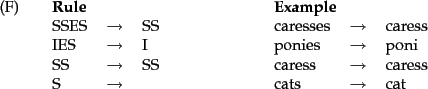
\includegraphics[scale=0.45]{pics/porter.png}
\end{figure}

Ejemplo: $d$ = Me gustan los lenguajes humanos y los lenguajes de programación $=>$ Me gustan los lenguaj y los program lenguaj\footnote{\url{http://9ol.es/porter_js_demo.html}}

El vocabulario del documento $d$ después de eliminar stopwords y realizar stemming:

\begin{table}
\centering
\begin{tabular}{c|c}
\hline
termId & value \\
\hline
t1 & human \\
t2 & languag \\
t3 & program\\
\hline
\end{tabular}
\end{table}


\paragraph{Lematización}

\begin{itemize}
   \item Otra estrategia de normalización de términos.
   \item También transforma las palabras en sus raíces.
   \item Realiza un análisis morfológico utilizando diccionarios de referencia (tablas de búsqueda) para crear clases de equivalencia entre \emph{tipos}.
   \item Por ejemplo, para el token \emph{estudios}, una regla de stemming devolvería el término \emph{estudi}, mientras que a través de la lematización obtendríamos el término \emph{study}\footnote{\url{https://blog.bitext.com/what-is-the-difference-between-stemming-and-lemmatization/}}.
\end{itemize}

\subsection{Ley de Zipf}
\begin{itemize}
   \item La Ley de Zipf, propuesta por \emph{George Kingsley Zipf} en \cite{zipf1935}, es una ley empírica sobre la frecuencia de los términos dentro de una colección de documentos (\textbf{corpus}).
   \item Establece que la frecuencia $f$ de un término en un corpus es inversamente proporcional a su posición $r$ en una tabla de frecuencia ordenada:
   \begin{equation}
      f = \frac{cf}{r^{\beta}}
   \end{equation}
   \item Donde $cf$ es una constante dependiente de la colección y $\beta > 0$ es un factor de decaimiento.
   \item Si $\beta = 1$, entonces $f$ sigue exactamente la Ley de Zipf; de lo contrario, sigue una distribución similar a la de Zipf.
   \item La ley se relaciona con el principio del mínimo esfuerzo. A menudo utilizamos pocas palabras para expresar ideas.
   \item La Ley de Zipf es un tipo de distribución de ley de potencia (distribuciones de cola larga).
\end{itemize}

\begin{figure}[h!]
	\centering
	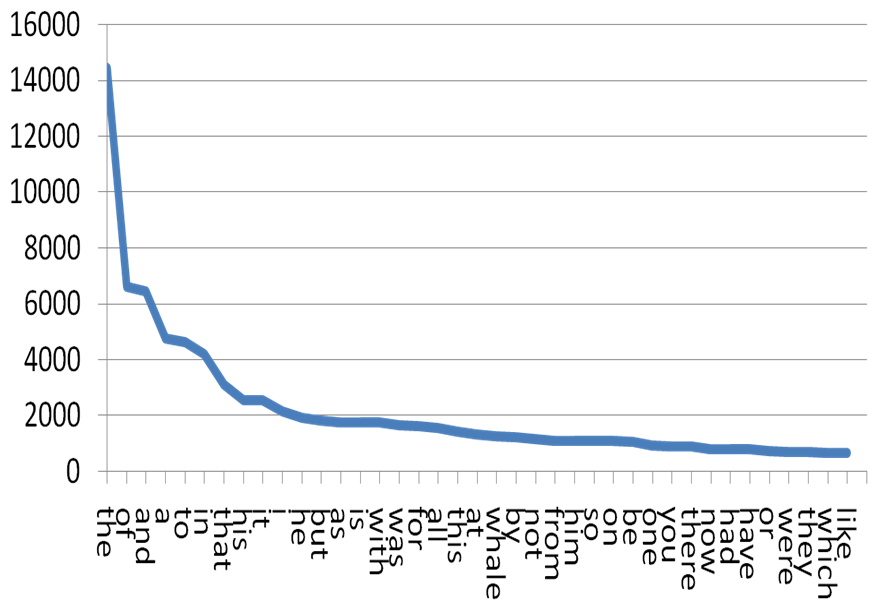
\includegraphics[scale=0.5]{pics/zipf1.png}
	\caption{Ley de Zipf}
\end{figure}

\begin{itemize}
   \item Si trazamos un gráfico de $log$-$log$, obtenemos una línea recta con una pendiente de $-\beta$.
   \item Enumerar las palabras más frecuentes de un corpus se puede utilizar para construir una lista de \emph{stopwords}.
\end{itemize}
\subsection{Listas de publicaciones y el índice invertido}
Sea $D$ una colección de documentos y $V$ el vocabulario de todos los términos extraídos de la colección:

\begin{itemize}
\item La lista de publicaciones de un término es la lista de todos los documentos donde el término aparece al menos una vez. Los documentos se identifican por sus identificadores.
\item Un índice invertido es una estructura de datos tipo diccionario que mapea los términos $t_{i} \in V$ con sus listas de publicaciones correspondientes.
\begin{displaymath}
<\text{término}> \rightarrow <\text{idDocumento}>^*
\end{displaymath}
\end{itemize}

\begin{figure}[h!]
\centering
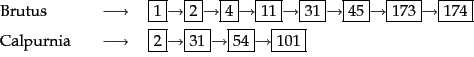
\includegraphics[scale=0.6]{pics/invFile.png}
\caption{Índice invertido}
\end{figure}

\subsection{Motores de búsqueda web}

Un motor de búsqueda es un sistema de recuperación de información diseñado para buscar información en la web (satisfacer necesidades de información) \cite{manning2008}. Sus componentes básicos son:

\begin{itemize}
\item Rastreador: un robot que navega por la web según una estrategia definida. Por lo general, comienza navegando por un conjunto de sitios web iniciales y continúa navegando a través de sus enlaces.
\item Indexador: se encarga de mantener un índice invertido con el contenido de las páginas recorridas por el rastreador.
\item Procesador de consultas: se encarga de procesar las consultas de los usuarios y buscar en el índice los documentos más relevantes para una consulta.
\item Función de clasificación: la función utilizada por el procesador de consultas para clasificar los documentos indexados en la colección por relevancia según una consulta.
\item Interfaz de usuario: recibe la consulta como entrada y devuelve los documentos clasificados por relevancia.
\end{itemize}

\begin{figure}[h!]
\centering
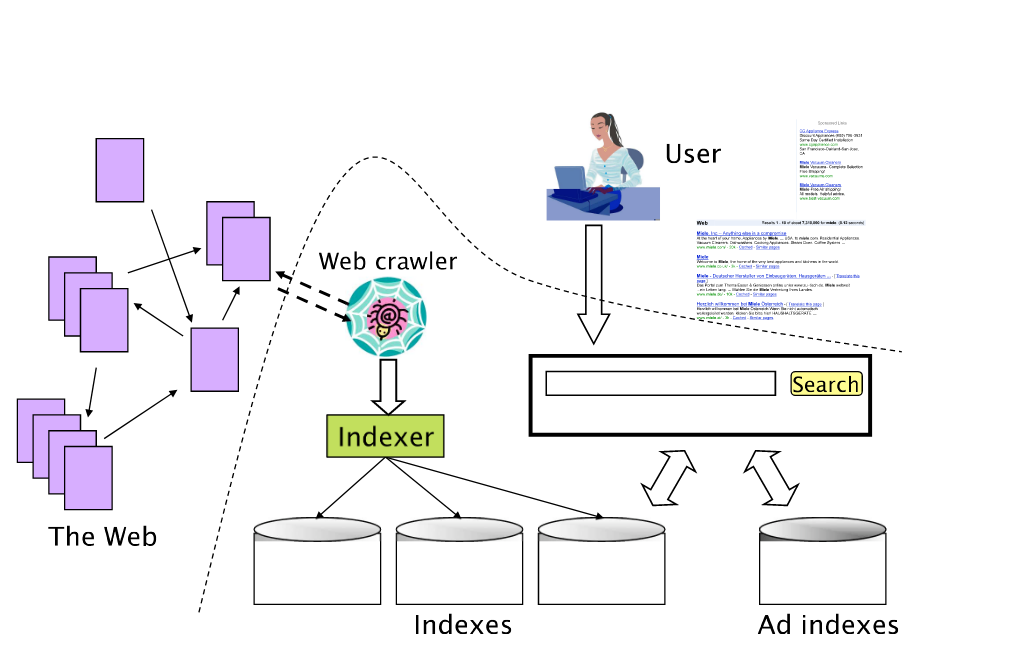
\includegraphics[scale=0.25]{pics/searchengine.png}
\caption{Los diversos componentes de un motor de búsqueda web \cite{manning2008}.}
\end{figure}
\section{El modelo de espacio vectorial}

\begin{itemize}
\item Para clasificar consultas o medir la similitud entre dos documentos, necesitamos una métrica de similitud.
\item Los documentos pueden ser \textit{representados} como vectores de términos, donde cada término es una dimensión del vector \cite{salton1975vector}.
\item Documentos con diferentes palabras y longitudes residirán en el mismo espacio vectorial.
\item Este tipo de representaciones se llaman \emph{Bolsa de Palabras} (Bag of Words).
\item En las representaciones de bolsa de palabras, se pierde el orden de las palabras y la estructura lingüística de una oración.
\item El valor de cada dimensión es un peso que representa la relevancia del término $t_{i}$ en el documento $d$.
\begin{equation}
d_{j} \rightarrow \overrightarrow{d_{j}}=(w(t_{1},d_{j}),...,w(t_{|V|},d_{j}))
\end{equation}
\item ¿Cómo podemos modelar la información que aporta un término a un documento?
\end{itemize}

\paragraph{Frecuencia de Término - Frecuencia Inversa de Documento}

\begin{itemize}
\item Sea $tf_{i,j}$ la frecuencia del término $t_{i}$ en el documento $d_{j}$.
\item Un término que ocurre 10 veces debería proporcionar más información que uno que ocurre solo una vez.
\item ¿Qué ocurre cuando tenemos documentos que son mucho más largos que otros?
\item Podemos normalizar dividiendo por la frecuencia máxima del término en el documento.
\begin{displaymath}
ntf_{i,j}=\frac{tf_{i,j}}{\max_i (tf_{i,j})}
\end{displaymath}
\item ¿Un término que ocurre en muy pocos documentos proporciona más o menos información que uno que ocurre varias veces?
\item Por ejemplo, el documento \emph{El respetado alcalde de Pelotillehue}. El término \emph{Pelotillehue} ocurre en menos documentos que el término \emph{alcalde}, por lo que debería ser más descriptivo.
\item Sea $N$ el número de documentos en la colección y $n_{i}$ el número de documentos que contienen el término $t_{i}$, definimos la frecuencia inversa de documento ($idf$) de $t_{i}$ de la siguiente manera:
\begin{displaymath}
idf_{t_{i}}= \log_{10}\left(\frac{N}{n_{i}}\right)
\end{displaymath}
\item Un término que aparece en todos los documentos tendría $idf=0$, y uno que aparece en el $10\%$ de los documentos tendría $idf=1$.
\item El modelo de puntuación $tf$-$idf$ combina las puntuaciones de $tf$ e $idf$, y resulta en los siguientes pesos $w$ para un término en un documento:
\begin{displaymath}
w(t_{i},d_{j})=tf_{i}\times \log_{10}\left(\frac{N}{n_{i}}\right)
\end{displaymath}
\item Las consultas de los motores de búsqueda también pueden ser modeladas como vectores. Sin embargo, en promedio, las consultas suelen tener entre 2 y 3 términos. Para evitar tener demasiadas dimensiones nulas, los vectores de consulta pueden suavizarse de la siguiente manera:
\begin{displaymath}
w(t_{i},d_{j})=(0.5+0.5\times tf_{i,j})\log_{10}\left(\frac{N}{n_{i}}\right)
\end{displaymath}
\end{itemize}

\subsection{Similitud entre vectores}
\begin{itemize}
\item Representar consultas y documentos como vectores permite calcular su similitud.
\item Un enfoque podría ser utilizar la distancia euclidiana.
\item El enfoque común es calcular el coseno del ángulo entre los dos vectores.
\item Si ambos documentos son iguales, el ángulo sería $0$ y su coseno sería $1$. Por otro lado, si son ortogonales, el coseno es $0$.
\item La similitud del coseno se calcula de la siguiente manera:
\begin{displaymath}
\text{similitud del coseno}(\vec{d}{1},\vec{d}{2})= \frac{\vec{d}{1}\cdot \vec{d}{2}}{|\vec{d}{1}|\times|\vec{d}{2}|} = \frac{\sum_{i=1}^{|V|}(w(t_{i},d_{1})\times w(t_{i},d_{2}))}{\sqrt{\sum_{i=1}^{|V|} w(t_{i},d_{1})^2}\times \sqrt{\sum_{i=1}^{|V|} w(t_{i},d_{2})^2}}
\end{displaymath}
\item Esto se llama incorrectamente "distancia del coseno". En realidad, es una métrica de similitud.
\item Observa que la similitud del coseno normaliza los vectores por su norma euclidiana $||\vec{d}||_{2}$.

\end{itemize}

\begin{figure}[h!]
\centering
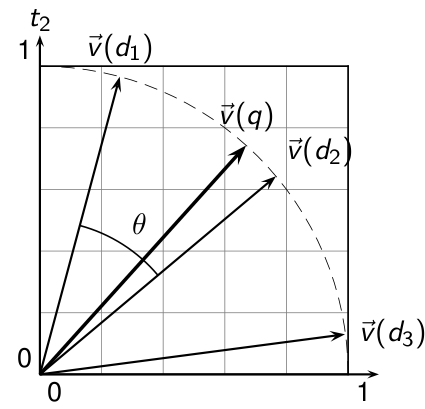
\includegraphics[scale=0.5]{pics/cos.png}
\caption{Similitud del coseno.}
\end{figure}
\paragraph{Ejercicio}
\begin{itemize}
\item Supongamos que tenemos $3$ documentos formados a partir de las siguientes secuencias de términos: \
$d_{1}\rightarrow t_{4}t_{3}t_{1}t_{4}$ \
$d_{2}\rightarrow t_{5}t_{4}t_{2}t_{3}t_{5}$ \
$d_{3}\rightarrow t_{2}t_{1}t_{4}t_{4}$ \
\item Construye una matriz término-documento de dimensiones $5\times3$ utilizando pesos simples de $tf$-$idf$ (sin normalización).
\item Recomendamos que primero construyas una lista con el número de documentos en los que aparece cada término (útil para calcular los valores de $idf$).
\item Luego, calcula los valores de $idf$ para cada término.
\item Rellena las celdas de la matriz con los valores de $tf$-$idf$.
\item ¿Cuál es el documento más cercano a $d_{1}$?
\end{itemize}

 \begin{table}[htbp]
 \centering
\begin{tabular}{|l|r|r|r|}
\hline
 & \multicolumn{1}{l|}{d1} & \multicolumn{1}{l|}{d2} & \multicolumn{1}{l|}{d3} \\ \hline
t1 & 0.176 & 0.000 & 0.176 \\ \hline
t2 & 0.000 & 0.176 & 0.176 \\ \hline
t3 & 0.176 & 0.176 & 0.000 \\ \hline
t4 & 0.000 & 0.000 & 0.000 \\ \hline
t5 & 0.000 & 0.954 & 0.000 \\ \hline
\end{tabular}
\caption{Matriz tf-idf}
\end{table}

\section{Agrupamiento de Documentos}

\begin{itemize}
\item ¿Cómo podemos agrupar documentos que son similares entre sí?
\item El agrupamiento es el proceso de agrupar documentos que son similares entre sí.
\item Cada grupo de documentos se llama \emph{cluster} o grupo.
\item En el agrupamiento, intentamos identificar grupos de documentos en los que la similitud entre documentos en el mismo grupo se maximiza y la similitud de documentos en diferentes grupos se minimiza.
\begin{figure}[h!]
\centering
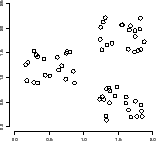
\includegraphics[scale=0.6]{pics/cluster.png}
\caption{ Conjunto de documentos donde los grupos se pueden identificar claramente.}
\end{figure}
\item El agrupamiento de documentos permite identificar temas en un corpus y reducir el espacio de búsqueda en un motor de búsqueda, es decir, el índice invertido se organiza según los grupos.
\item K-means es un algoritmo de agrupamiento simple que recibe el número de grupos $k$ como parámetro.
\item El algoritmo se basa en la idea de \emph{centroide}, que es el vector promedio de los documentos que pertenecen al mismo grupo.
\item Sea $S$ un conjunto de vectores bidimensionales ${3,6}, {1,2}, {5,1}$, el centroide de $S$ es ${(3+1+5)/3,(6+2+1)/3} = {3,3}$.

\end{itemize}

\subsection{K-Means}
\begin{enumerate}
\item Comenzamos con $k$ centroides aleatorios.
\item Calculamos la similitud entre cada documento y cada centroide.
\item Asignamos cada documento a su centroide más cercano formando un grupo.
\item Se recalculan los centroides de acuerdo a los documentos asignados a ellos.
\item Este proceso se repite hasta la convergencia.
\end{enumerate}

\begin{figure}[h!]
\centering
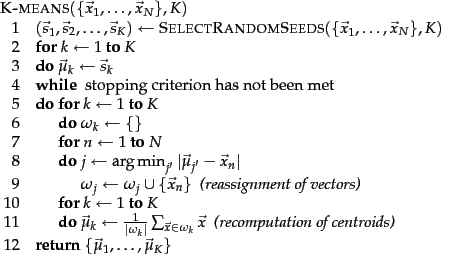
\includegraphics[scale=0.6]{pics/kmeans.png}
\caption{ Algoritmo K-means}
\end{figure}

\section{Conclusiones y Conceptos Adicionales}
\begin{itemize}
\item Representar documentos como vectores es fundamental para calcular similitudes entre pares de documentos.
\item Los vectores de "bag of words" carecen de estructura lingüística.
\item Los vectores de "bag of words" son de alta dimensionalidad y dispersos.
\item Los n-gramas de palabras pueden ayudar a capturar expresiones de múltiples palabras (por ejemplo, New York $=>$ new\_york)
\item Los sistemas modernos de recuperación de información van más allá de la similitud de vectores (PageRank, Retroalimentación de relevancia, Minería de registros de consultas, Grafo de conocimiento de Google, Aprendizaje automático).
\item La recuperación de información y la minería de textos se preocupan menos por la estructura lingüística y más por producir algoritmos rápidos y escalables \cite{jacobbook}.
\end{itemize}



\bibliography{bio}
\bibliographystyle{apalike}

\end{document}
